
%\begin{document}

\section{mmbucket - Multi-dimensional Uniform Bucket Partition\label{sect:mmbucket}}
\index{mmbucket@mmbucket}

Segment numerical values in multiple fields specified at \verb|f=| into equal sized buckets. For example, set \verb|f=a,b,c| and \verb|n=5|, \hyperref[sect:mbucket]{mbucket} command segments fields \verb|a,b,c| into 5 equal buckets. Whereas mmbucket allocate items \verb|a,b,c| into 3 dimensional space for each bucket (bucket number becomes $5^3=125$ ) such that each interval is distributed as evenly as possible. 


\subsection*{Format}
\verb|mmbucket f= n= [F=] [k=] [O=] [-ms] [-r]| 
\hyperref[sect:option_i]{[i=]}
\hyperref[sect:option_o]{[o=]}
\hyperref[sect:option_bufcount]{[bufcount=]} 
\hyperref[sect:option_assert_diffSize]{[-assert\_diffSize]}
\hyperref[sect:option_assert_nullkey]{[-assert\_nullkey]}
\hyperref[sect:option_assert_nullin]{[-assert\_nullin]}
\hyperref[sect:option_assert_nullout]{[-assert\_nullout]}
\hyperref[sect:option_nfn]{[-nfn]} 
\hyperref[sect:option_nfno]{[-nfno]}  
\hyperref[sect:option_x]{[-x]}
\hyperref[sect:option_q]{[-q]}
\hyperref[sect:option_option_tmppath]{[tmpPath=]}
\verb|[--help]|
\verb|[--helpl]|
\verb|[--version]|\\

\subsection*{Parameters}
\begin{table}[hbt]
%\begin{center}
{\small
\begin{tabular}{ll}
\verb|f=|    & Values in this field(s) (multiple fields can be specified) is(are) partitioned.  \\
             & When there are multiple fields, the number of dimensions is determined based on equal number of buckets. \\
             & When 1 field is specified, the result is the same as using \verb|mbucket|. \\
             & \verb|-x,-nfn| options can be used to specify field number (0〜).\\
\verb|n=|    & Each bucket size corresponds to a field specified at \verb|f=|. \\
		& The number of items defined here is the same as the number of fields specified at \verb|f=|. \\
		& However, if there is only 1 number specified, the same partition number is applied to other field.  \\
\verb|F=|    & Ouput format [default value: 1]\\
             & Output format of bucket name.\\
             & 0: Display bucket number. \\
             & 1: Display value range of buckets. \\
             & 2: Display both bucket number and value range. \\
\verb|k=|    & Unique key field(s) (multiple fields can be specified) to retrieve rows of data for partitioning into buckets. \\
\verb|O=|    & Specifies the output file with numeric range of each bucket from the items specified in the \verb|f=| parameter.  \\
\verb|-ms|   & When partitioning buckets for each field sequentially, the first item is changed multiple times \\
		& during the bucket partition trial. \\
             & For further information, refer to the "Introduction to Algorithms" to find out the best possible solution. \\
\verb|-r|    & Display bucket number in reverse order. \\
\end{tabular} 
}
\end{table} 

\subsection*{Examples}
\subsubsection*{Example 1: Basic Example}

Partition the number of records in column \verb|x,y| into two multi-dimentional equal subsets. At the same time, save the numeric range of each bucket in the file named \verb|rng.csv|.


\begin{Verbatim}[baselinestretch=0.7,frame=single]
$ more dat1.csv
id,x,y
A,2,7
B,6,7
C,5,6
D,7,5
E,6,4
F,1,3
G,3,3
H,4,2
I,7,2
J,2,1
$ mmbucket f=x:xb,y:yb n=2,2 O=rng.csv i=dat1.csv o=rsl1.csv
calculating on dimension ... #0 #1 done. VAR=30 updated!
calculating on dimension ... #0 #1 done. VAR=28 updated!
calculating on dimension ... #0 #1 done. VAR=28
#END# kgmbucket O=rng.csv f=x:xb,y:yb i=dat1.csv n=2,2 o=rsl1.csv
$ more rsl1.csv
id,x,y,xb,yb
A,2,7,1,2
B,6,7,2,2
C,5,6,2,2
D,7,5,2,2
E,6,4,2,1
F,1,3,1,1
G,3,3,1,1
H,4,2,2,1
I,7,2,2,1
J,2,1,1,1
$ more rng.csv
fieldName,bucketNo,rangeFrom,rangeTo
x,1,,3.5
x,2,3.5,
y,1,,4.5
y,2,4.5,
\end{Verbatim}
\subsubsection*{Example 2: Outupt Format}

Partition the number of records in column \verb|x,y| into two multi-dimentional equal subsets based on the \verb|id| field. The output format shall display the both the bucket number and numeric range.


\begin{Verbatim}[baselinestretch=0.7,frame=single]
$ more dat2.csv
id,x,y
A,2,7
A,6,7
A,5,6
B,7,5
B,6,4
B,1,3
C,3,3
C,4,2
C,7,2
C,2,1
$ mmbucket k=id f=x:xb,y:yb n=2,2 F=2 i=dat2.csv o=rsl2.csv
calculating on dimension ... #0 #1 done. VAR=3 updated!
calculating on dimension ... #0 #1 done. VAR=3
calculating on dimension ... #0 #1 done. VAR=3 updated!
calculating on dimension ... #0 #1 done. VAR=3
calculating on dimension ... #0 #1 done. VAR=6 updated!
calculating on dimension ... #0 #1 done. VAR=6
#END# kgmbucket F=2 f=x:xb,y:yb i=dat2.csv k=id n=2,2 o=rsl2.csv
$ more rsl2.csv
id%0,x,y,xb,yb
A,2,7,1:_3.5,2:6.5_
A,6,7,2:3.5_,2:6.5_
A,5,6,2:3.5_,1:_6.5
B,7,5,2:3.5_,2:4.5_
B,6,4,2:3.5_,1:_4.5
B,1,3,1:_3.5,1:_4.5
C,3,3,1:_3.5,2:1.5_
C,4,2,2:3.5_,2:1.5_
C,7,2,2:3.5_,2:1.5_
C,2,1,1:_3.5,1:_1.5
\end{Verbatim}

\subsection*{Overview of algorithm\footnote{This algorithm is developed by Professor Naoki Kato (Kyoto University, Graduate School of Engineering).}}

Assuming data set $D$ consists of two columns $A,B$ with numerical values. The numeric range in column $A$ and $B$ is divided into $K$ bits and $L$ bits respectively. \verb|mmbucket| determines how to divide the data equally into segments (buckets). Dispersion is used as a basis to measure the uniformity of distribution.  The variance value minimizes the number of buckets partitions based on the heuristics described below, which is not guaranteed to be optimal. The algorithm is described as follows. \\

\begin{enumerate}
\item Partition data in field $A$ by \hyperref[sect:mbucket]{one dimensional uniform partition}. \\
\item Determine the partition of $A$ from step 1, partition the range of numerical values in $B$ into buckets. The evaluation criteria for two-dimensional bucket partition is based on the partitions. Dynamic programming and one-dimensional bucket partition is used to divide buckets in to equal sized partitions.\\
\item Next, using the partitions of $B$ obtained from step 2, partition the range of numerical values in $A$. As in step 2, the values of two dimensional bucket partition is used as an evaluation criteria. \\
\item Repeat step 2 and 3 recursively until improvement of variance is minute.\\
\item Return partition output. \\
\end{enumerate}

During implementation, when $A$ and $B$’s parts are switched in step 1, the solution returns the one with more optimal results. The same algorithm applies to uniform buckets partition for three or more dimensions.


\subsection*{Comparison of mbucket and mmbucket}

The following explains how multi-dimensional bucket partition operates compared to one-dimensional bucket partition. 
Table \ref{tbl:mmbucket_indata} shows two columns x and y, with 10 rows data of id from A to J. 

Using this data, each of x and y is divided into two partitions, thus create a total of four buckets as shown in Figure \label{fig:mmbucket_1dim}. The results of one-dimensional bucket partition on x and y is shown in column x1, y1. In addition, the results of multi-dimensional bucket partition is shown in column x2 and y2 as displayed in Figure \label{fig:mmbucket_2dim}. \\

Variance (sum of squares of each bucket : for more information, refer to formulation of \hyperref[sect:mbucket]{mbucket}) of one dimensional bucket partition is computed as $Var_a'=1^2+4^2+4^2+1^2=34$, and $Var_b'=1^2+3^2+3^2+3^2=28$ for two-dimensional bucket partition. During one-dimensional bucket partition x and y is treated independently to optimize solution with minimal variance (i.e. each is divided into 5). The solution of one dimensional bucket partition is inferior to two-dimensional bucket partition.
One dimensional bucket partition can be improved by using the multi-dimensional bucket partition. However, multi-dimensional partition requires a lot of CPU time dependent on the contents of the data.


\begin{table}[hbt]
\begin{center}
 \caption{Sample result of output from mbucket,mmbucket\label{tbl:mmbucket_indata}}
{\footnotesize
 \begin{tabular}{c|c|c|c|c|c|c}
  \hline
  \multicolumn{3}{c|}{Data} & \multicolumn{2}{|c|}{mbucket} & \multicolumn{2}{|c}{mmbucket} \\
\hline
id & x & y & x1 & y1 & x2 & y2 \\
\hline
A & 2 & 7 & 1 & 2 & 1 & 2 \\
B & 6 & 7 & 2 & 2 & 2 & 2 \\
C & 5 & 6 & 2 & 2 & 2 & 2 \\
D & 7 & 5 & 2 & 2 & 2 & 2 \\
E & 6 & 4 & 2 & 2 & 2 & 1 \\
F & 1 & 3 & 1 & 1 & 1 & 1 \\
G & 3 & 3 & 1 & 1 & 1 & 1 \\
H & 4 & 2 & 1 & 1 & 2 & 1 \\
I & 7 & 2 & 2 & 1 & 2 & 1 \\
J & 2 & 1& 1 & 1 & 1 & 1 \\ 
\hline
 \end{tabular}
}
\end{center}
\end{table}

\begin{figure}[htbp]
\begin{center}
\begin{tabular}{c}

\begin{minipage}{0.45\hsize}
\begin{center}
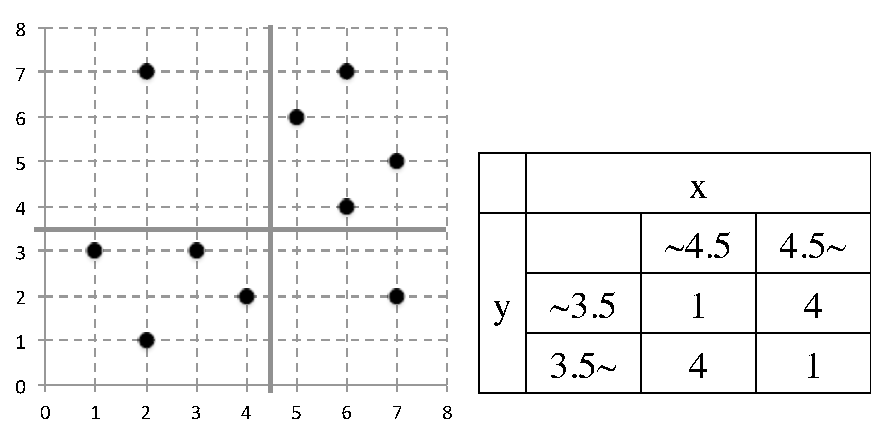
\includegraphics[scale=.50]{figure/mmbucket/split_mbucket.eps}
\end{center}
\caption{One-dimensional partition (mbucket)×2\label{fig:mmbucket_1dim}}
\end{minipage}

\begin{minipage}{0.45\hsize}
\begin{center}
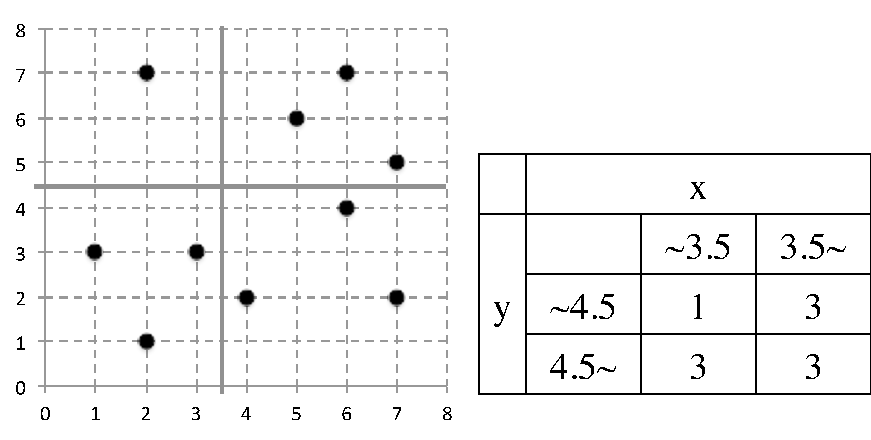
\includegraphics[scale=.50]{figure/mmbucket/split_mmbucket.eps}
\end{center}
\caption{Two-dimensional partition (mmbuket)\label{fig:mmbucket_2dim}}
\end{minipage}

\end{tabular}
\end{center}
\end{figure}


%\begin{figure}[hbt]
%\begin{center}
%\includegraphics[width=20cm,bb=0 0 738 430]{./img/bucket_var.JPG}
%\caption{1次元分割×2による分割と2次元分割による分割の比較}
%\end{center}
%\end{figure}

\subsection*{Precision experiment using on variety of fields}

The following compares the precision of mmbucket and mbucket using real data collected by \href{http://www.pmel.noaa.gov/tao/}{Tropical Atmosphere Ocean (TAO) Project}. The project is designed for the study of year-to-year climate variations related to El Nino the Southern Oscillation (ENSO), and provides provides in-situ data collection of high quality oceanographic and surface meteorological data for monitoring, forecasting, and understanding of climate swings associated with El Nino and La Nina.  Snapshot of the data is shown in the following table. \\



\begin{table}[hbt]
\begin{center}
\caption{Data set used for precision experiment }
{\footnotesize
%\begin{tabular}{p{2em}|p{2.5em}|p{2em}|p{3em}|p{3.5em}|p{4em}|p{4.5em}|p{4.5em}|p{3.5em}|p{3.5em}|p{4.5em}|p{2.5em}}\hline
\begin{tabular}{l|l|l|l|l|l|l|l|l|l|l|l}\hline
%obs  (観測id) & year (年)&month (月)&day (日)&date (日付) &latitude (緯度)&longitude (経度)&zonwinds (東西風速)	&merwinds (南北風速)&humidity (湿度)&air\_temp. (気温)&sstemp (海面温度) \\ \hline
id & year & month & day & date & latitude & longitude & zonwinds & merwinds & humidity & air\_temp. &sstemp \\ \hline
4060 & 93 &5 & 9 & 930509 & -0.02 & -109.96 & -2.1 & 2.1 & 81.2 & 26.8 & 27.02\\
4061 & 93 & 5 & 10 & 930510 & -0.02 & -109.96 & -3.4 & 1.4 & 84.2 & 26.95 & 26.91\\
4062 & 93 & 5 & 11 & 930511 & -0.02 & -109.96 & -3.8 & 2.2 & 84.9 & 26.98 & 26.78\\
4063 & 93 & 5 & 12 & 930512 & -0.02 & -109.96 & -3 & 1.5 & 86.9 & 26.93 & 26.74\\
4064 & 93 & 5 & 13 & 930513 & -0.02 & -109.96 & -4.5 & 1.9 & 87.6 & 27.01 & 26.82\\
4065 & 93 & 5 & 14 & 930514 & -0.02 & -109.96 & -5    & 1.3 & 85.6 & 26.96 & 26.68\\
\hline
\end{tabular}
\\
%latitude:緯度, longitude:経度, zonwinds:東西風速, merwinds:南北風速, humidity:湿度, air\_temp.:気温, sstemp:海面温度
}
\end{center}
\end{table}

The precision experiment uses attributes with numeric values (7 attributes from latitude to sea surface temperature) for bucket partition. The number of record rows is 93,935. Statistics for each attribute is shown in Table 3. "Types of data values" significantly affects computation time of bucket partition.


\begin{table}[hbt]
\begin{center}
\caption{Various statistics of numerical data}
{\footnotesize
\begin{tabular}{c|c|c|c|c|c|c|c} \hline
Measurement & Latitude& Longitude & Zonal wind & North-south wind & Humidity & Temp & Sea surface temp\\ \hline
Type & 482& 924& 228& 206& 385& 1104& 1201\\
Arithmetic average& 0.305& -70.8& -3.35& -0.046& 81.3& 27.1& 27.9\\
Standard deviation & 4.77& 128.7& 3.42& 3.021& 5.28& 1.674& 1.87\\
Minimum & -8.33& -180& -10.7& -10.6& 52.1& 17.5& 18.2\\
Mean & 0.01& -125& -4.1& -0.1& 81.3& 27.5& 28.4\\
Maximum& 9.05& 170.0& 14.3& 13& 99.9& 31.5& 31.0\\ \hline
\end{tabular}
}
\end{center}
\end{table}

The comparison of variance for one-dimensional bucket partition (mbucket) and two-dimensional bucket partition (mmbucket) based on a total of 21 combinations from the 7 attributes are distributed into two columns as shown in Table \ref{tbl:mmbucket_table1}. 

For example, the first row shows the comparison results of bucket partition on “temperature × humidity”, the variance of mbucket is 408274409 and the variance of mmbucket is 406438211, resulting in the ratio of (mmbucket / mbucket) 0.996. The ratio is shown for partitions of 10×10,15×15 and 20×20. The results differs according to the combination of attributes, there are minimal improvements in some combinations such as "humidity × zonal wind speed", improvements can be seen at “latitude x longtitude (15 x 15) with an improvement in accuracy of 19\% (1-0.81).

\begin{table}[hbt]
\begin{center}
\caption{Comparison of two-dimensional partition accuracy of mbucket and mmbucket\label{tbl:mmbucket_table1}}
{\footnotesize
\begin{tabular}{c|c||c|c|c|c|c|c}
\hline
% plastexにてmultirowはNG
%\multirow{2}{*}{項目1} & \multirow{2}{*}{項目2} & \multicolumn{2}{|c|}{分散値(5×5分割)} & \multicolumn{4}{|c}{分散値の比(mmbucket/mbucket)} \\  \cline{3-4}  \cline{5-8}
%                       &  & mbucket  & mmbucket & 5×5 &	10×10 & 15×15 & 20×20  \\ \hline\hline
            &          & \multicolumn{2}{|c|}{Variance (5×5 partition)} & \multicolumn{4}{|c}{Comparison of variance (mmbucket/mbucket)} \\  \cline{3-4}  \cline{5-8}
Item 1       & Item 2    & mbucket  & mmbucket & 5×5  &10×10 &15×15 & 20×20\\ \hline\hline
Temperature        & Humidity     &408274409 &406438211 &0.996 &0.987 &0.988 &0.981 \\
            & Latitude     &374125463 &371258775 &0.992 &0.988 &0.982 &0.964 \\
            & Longitude     &490727955 &454663065 &0.927 &0.949 &0.946 &0.929 \\
            & North-south wind speed &396436813 &394724219 &0.996 &0.991 &0.993 &0.989 \\
            & Sea surface temperature &816199131 &747215787 &0.915 &0.897 &0.883 &0.862 \\
            & Zonal wind speed &382069455 &381225143 &0.998 &0.998 &0.997 &0.996 \\  \hline
Temperature        & Humidity     &368492959 &367941709 &0.999 &0.994 &0.994 &0.990 \\
            & Latitude     &372116309 &370591351 &0.996 &0.991 &0.993 &0.986 \\
            & North-south wind speed &355658757 &355658757 &1.000 &1.000 &1.000 &1.000 \\
            & Sea surface temperature &380382203 &379546293 &0.998 &0.991 &0.991 &0.983 \\
            & Zonal wind speed &357729819 &357697283 &1.000 &1.000 &1.000 &1.000 \\ \hline
Latitude        & Longtitude     &365459223 &361754113 &0.990 &0.923 &0.812 &0.816 \\
            & North-south wind speed &371478669 &370970251 &0.999 &0.988 &0.985 &0.982 \\
            & Sea surface temperature &392810425 &389589403 &0.992 &0.987 &0.979 &0.952 \\
            &  Zonal wind speed &364521077 &364406663 &1.000 &0.999 &0.991 &0.992 \\ \hline
Longtitude        & Latitude &414154185 &408431667 &0.986 &0.976 &0.976 &0.962 \\
            & Sea surface temperature &510979465 &463576537 &0.907 &0.945 &0.939 &0.934 \\
            & Zonal wind speed &400021527 &392710641 &0.982 &0.983 &0.982 &0.973 \\ \hline
North-south wind    & Sea surface temperature &393233841 &392432943 &0.998 &0.995 &0.994 &0.993 \\
            & Zonal wind speed &359290669 &359074015 &0.999 &1.000 &1.000 &0.997 \\ \hline
Sea surface temp    & Zonal wind speed &442877539 &438326669 &0.990 &0.988 &0.984 &0.986 \\ \hline
\end{tabular}
}
\end{center}
\end{table}
 
\subsection*{Speed Comparison}

Next, the experiments are carried out to compare the differences in speed by against different  number of partitions. The execution time is computed using the same data “temperature × sea surface temperature” and “latitude × longitude” with 5 to 40 partitions at increments of 5.  The results are shown in Table \ref{tbl:mmbucket_table2}. The execution time of \verb|mbucket| is consistent regardless of the number of partitions. However, more time is required to compute the number of partitions for two dimensional partitions. This is due to the fact that the algorithm is not efficient in selecting multidimensional orthogonal numeric range required by computation. The partition speed will be noted as possible improvements in the next version. 


\begin{table}[hbt]
\begin{center}
\caption{Sample results of mbucket,mmbucket \label{tbl:mmbucket_table2}}
{\footnotesize
\begin{tabular}{c|c|c|c|c}
\hline
& \multicolumn{2}{|c|}{Temperature×Sea Surface Temperature} & \multicolumn{2}{|c}{Latitude×Longtitude} \\ \hline
Number of buckets &mbucket &mmbucket &mbucket &mmbucket\\ \hline
5 &0.221 &2.21 &0.216 &0.67\\
10 &0.227 &3.90 &0.216 &1.67\\
15 &0.233 &10.4 &0.230 &3.28\\
20 &0.231 &26.1 &0.228 &7.13\\
25 &0.232 &32.9 &0.237 &13.3\\
30 &0.236 &46.7 &0.236 &11.4\\
35 &0.237 &62.3 &0.240 &15.2\\
40 &0.237 &80.1 &0.237 &25.8\\ \hline
\end{tabular}
}
\end{center}
\end{table}

\subsection*{Related Command}
\hyperref[sect:mbucket]{mbucket} : This command processes one-dimensional bucket partition for each field even when more than one field is specified.

%\end{document}


